\section{Project History}
Experience has taught the SKF project leaders that the state of application security is not adequate to ensure security. Primarily due to the lack of knowledge on secure programming \cite{skf_introduction}. As a result, SKF intended to solve this issue by developing a guide system in the form of an open source web application for developers to support them in developing secure software by design.

SKF has achieved this by adding security standards such as the ASVS and MASVS into their web application project management feature. Furthermore, contributors have added secure code examples for several popular programming languages and frameworks such as Java, PHP, go, ruby, nodejs, ASP.NET, flask and Django. The web application also has features such as hacking labs and a training platform to train developers, security pentesters and development operations (DevOps).

\section{Software Development Project Management}
SKF provides many features as discussed previously, this study however will only use SKF to design secure software through its project management feature. Specifically, MASVS security controls will be used to develop secure user authentication and user management throughout the requirements analysis, design, implementation and testing phases of the SDLC. 

\subsection{Requirements Analysis}
% Requirements - What do we want?
During the requirements' analysis phase the question, \say{What do we want?} is answered. From a security perspective, it is important to establish what security controls the software feature needs. In SKF, security requirements are defined when starting a new feature development sprint within a project.

\subsection{Design}
% Design - How do we get what we want?
After establishing what is required for the feature sprint, we seek to answer \say{How do we get what we want?}. Acceptance criteria can be defined based on the requirements established in the previous phase. During the design phase, developers come to understand what potential threats are introduced for the feature that is being developed and how they can be mitigated.

\subsection{Implementation}
% Implementation - Lets create what we want
After having defined what is required and how to get there, the implementation phase can begin. Based on the acceptance criteria code can be written not only focused on the functional requirement, but on the security requirement as well.

\subsection{Testing}
% Testing - Did we get what we wanted?
To ensure the security controls behave as they should, they need to be tested. MASVS-L1 allows for complete automated testing. Guidance on how to perform tests related to mobile security can be found in the MSTG. Links to the associated test for the security controls

\subsection{Setup and Installation on Linux}
SKF is completely free to use and open source. The entire source code is hosted on github. This allows organizations and developers to use SKF however they want, and even modify it to their needs. SKF hosts an online demo of their web application where users can get familiar with the web application. However, in a professional environment it is recommended to set up and install SKF on a personal server. 
d
SKF provides several installation options to host the web application. For this study, SKF was hosted on a local Arch Linux machine through docker. To run SKF on a Linux machine \textit{git}, \textit{docker}, \textit{docker-compose} and \textit{minikube} needs to be installed. On Arch Linux they can be installed throuch \textit{pacman}. Debian based distributions can install the required software with \textit{apt}. If docker is set up properly together with minikube, SKF can be cloned from its official repository on github. After cloning the repository, change directory into \verb|skf-flask| and run \verb|docker-compose up|. If no errors occur, the application can be accessed inside a browser on \textit{localhost} as seen in figure \ref{}. Step by step the process to install and setup SKF includes:

\begin{enumerate}
    \item Install \textit{docker, docker-compose}, and \textit{minikube}
    \item Clone SKF repository from \verb|https://github.com/blabla1337/skf-flask|
    \item Change directory into \verb|skf-flask|
    \item Run \verb|docker-compose up| inside the root folder
\end{enumerate}

\subsection{SKF Project Management}
When navigating to the project tabs in SKF, the user is shown a list of design pattern projects. Typically, the user wants to create their own project and set of requirements for a specific feature. To achieve this, the user can simply create a new project. The button is located in top right as seen in figure \ref{fig:skf-project}. This will bring the user to a page where the project details can be entered such the \emph{project name}, \emph{version} and \emph{description} as seen in figure \ref{fig:skf-new-project}. After the project is finished, it is added to the list of projects in the projects' page as seen in figure \ref{fig:skf-test-project}. 

When navigating to the created project, the user can create new requirements for a new feature or an existing feature by clicking the \textbf{Generate Requirements} button seen in figure \ref{fig:skf-project-features}. When generating new requirements for a feature, users can choose the \emph{checklist type}, \emph{verification level}, \emph{categories} and configure their sprint so that only the security requirements needed are generated. Lastly, the security expert system will ask whether the set of security requirements are to be added to an existing feature or a new one. Chapter 4 will discuss the complete process for the design of CheFeeds authentication and session management feature sprint

\begin{figure}
    \centering
    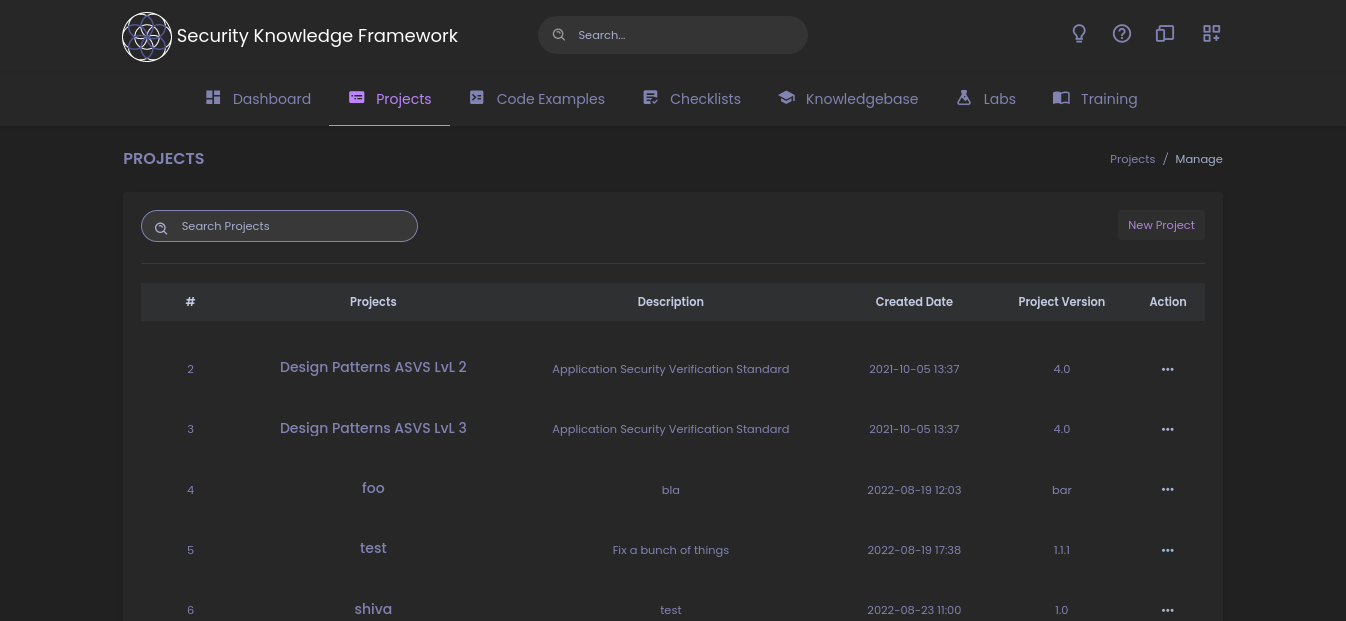
\includegraphics[width=0.5\textwidth]{chapter-3/skf-project.png}
    \caption{SKF Project}
    \label{fig:skf-project}
\end{figure}

\begin{figure}
    \centering
    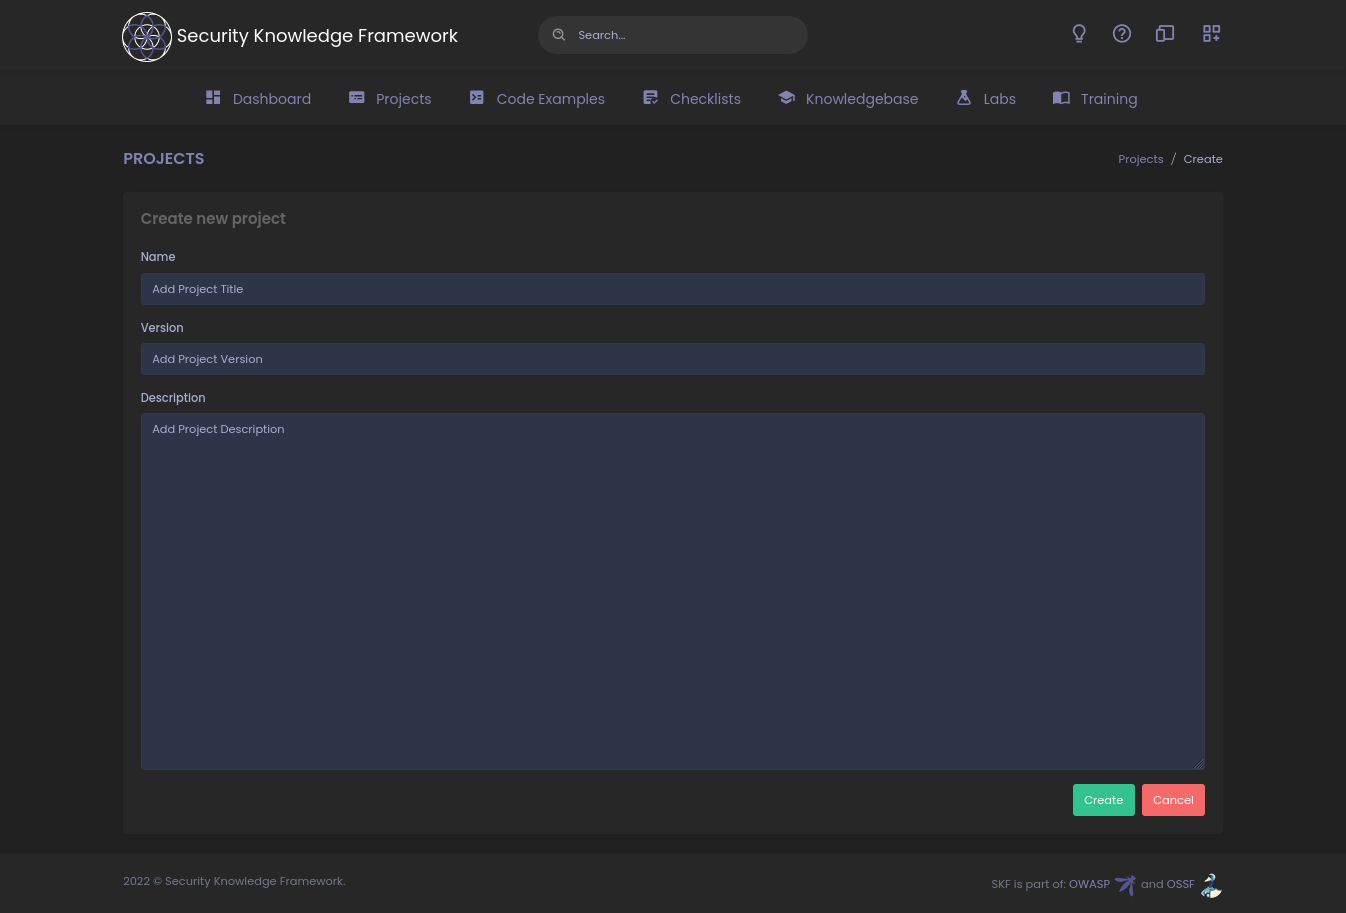
\includegraphics[width=0.5\textwidth]{chapter-3/skf-new-project-form}
    \caption{SKF New Project}
    \label{fig:skf-new-project}
\end{figure}

\begin{figure}
    \centering
    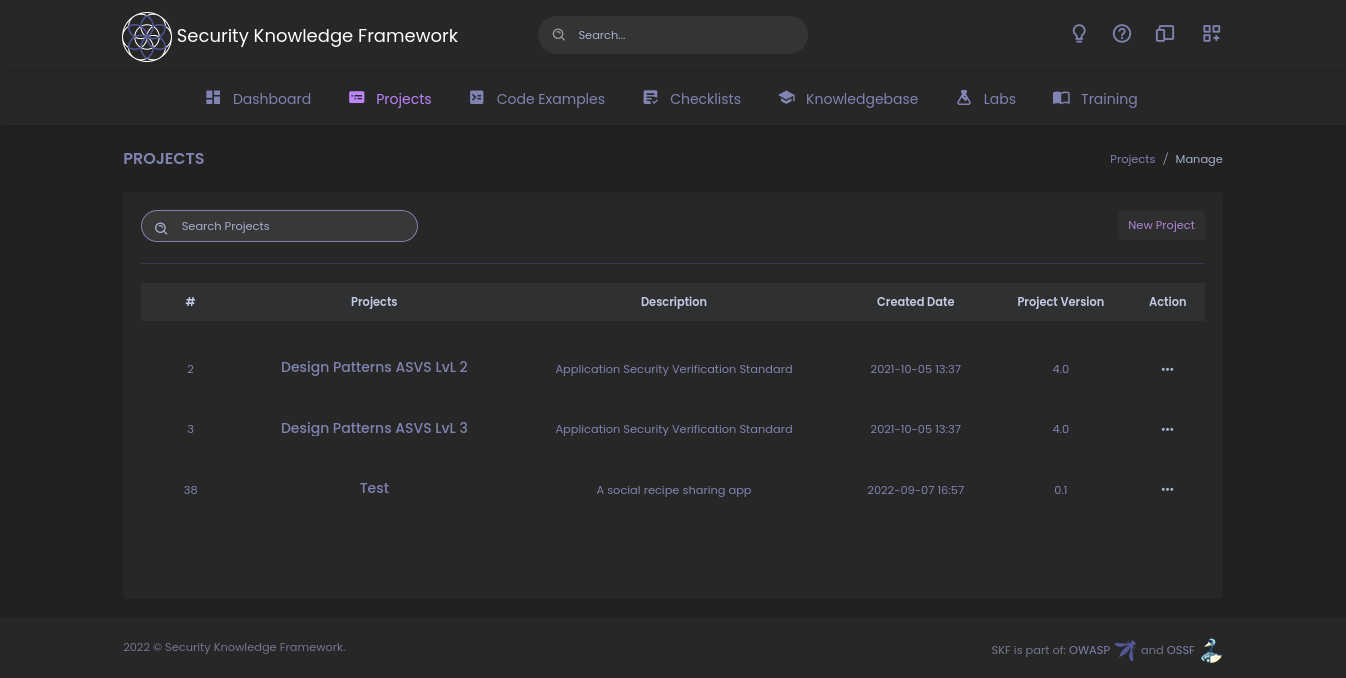
\includegraphics[width=0.5\textwidth]{chapter-3/skf-created-project}
    \caption{SKF new added project named \say{test}}
    \label{fig:skf-test-project}
\end{figure}

\begin{figure}
    \centering
    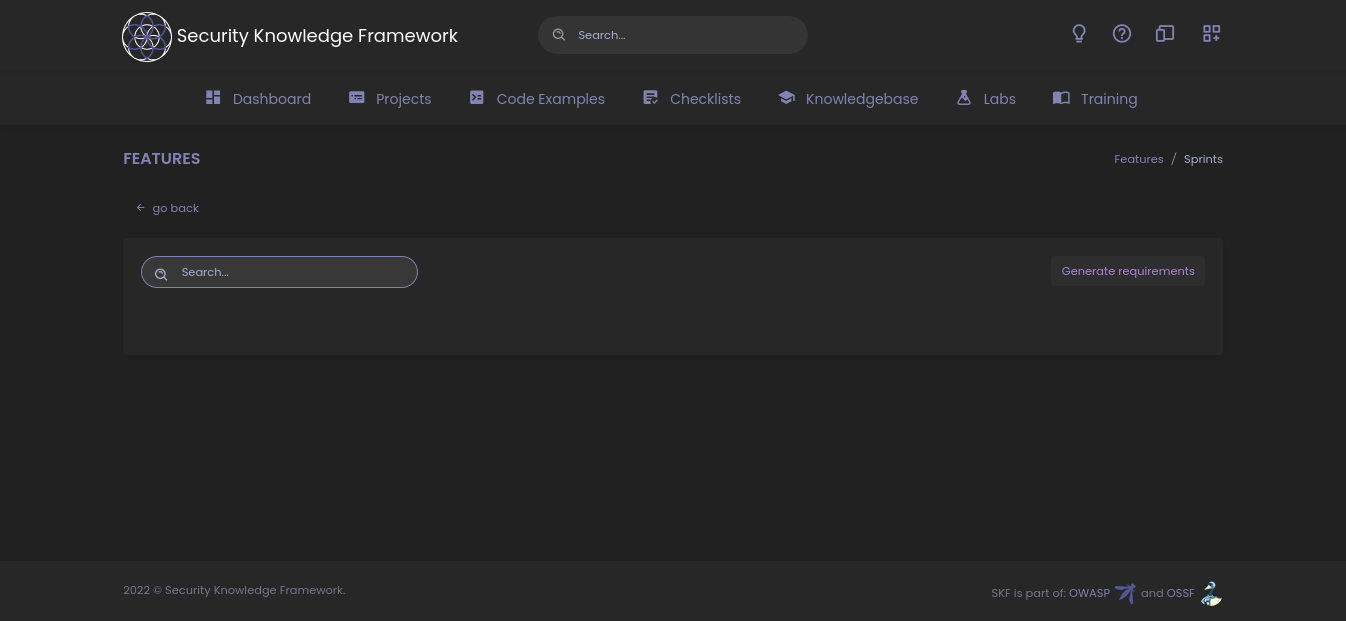
\includegraphics[width=0.5\textwidth]{chapter-3/skf-project-features-list}
    \caption{SKF project features}
    \label{fig:skf-project-features}
\end{figure}

\section{Alternative Solutions}
As far as the authors' knowledge goes, there are no solutions that are similar to SKF in its entirety. The best alternative solutions are the ASVS and MASVS and the related testing guide series from OWASP. SKF is unique as it provides a complete security framework and resource for organizations and developers who need to implement security. However, processes such as the OWASP Software Assurance Maturity Model (SAMM) or the Microsoft Security Lifecycle (SDL) may act as a complement to SKF. Both ensure that security activities are done throughout the whole SDLC. This section will briefly introduce them.

\subsection{OWASP Software Assurance Maturity Model}
The OWASP SAMM model provides a simple to use prescribed model which is fully defined, and measurable. SAMM assists organizations in analyzing the current software security practices, development of a security program in defined iterations, show gradual improvements in secure practices, and define and measure security-related activities. A complete overview of SAMMs model is illustrated in figure \ref{fig:samm-model}.

\begin{figure}
    \centering
    \caption{OWASP SAMM model}
    \label{fig:samm-model}
    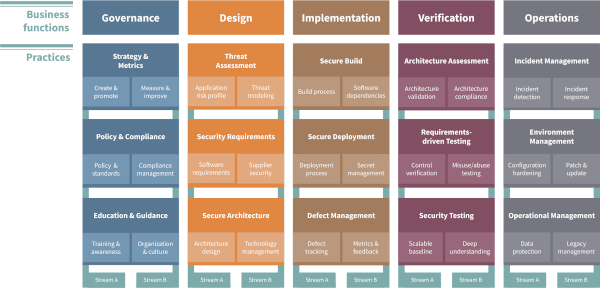
\includegraphics[width=0.5\textwidth]{chapter-4/OWASP-SAMM-model-600.png}
\end{figure}

\subsection{Microsoft Security lifecycle}
Microsofts SDL assists developers building highly secure software, address security compliance requirements, and reduce development costs. It keeps up to date with current technologies such as the cloud, Internet of Things, and artificial intelligence. The SDL includes a set of practices that support security assurance and compliance requirements. The set of practices included by the SDL are described in table \ref{tab:sdl-practices}.

\begin{table}
    \centering
    \caption{Microsoft SDL practices}
    \label{tab:sdl-practices}
    \begin{tabulary}{0.5\textwidth}{|l|L|}
        \hline
        \textbf{Practice \#} & \textbf{Description} \\
        \hline
        \textbf{Practice #1} & Provide Training \\
        \hline
        \textbf{Practice #2} & Define Security Requirements \\
        \hline
        \textbf{Practice #3} & Define Metrics and Compliance Reporting \\
        \hline
        \textbf{Practice #4} & Perform Threat Modeling \\
        \hline
        \textbf{Practice #5} & Establish Design Requirements \\
        \hline 
        \textbf{Practice #6} & Define and Use Cryptographic Standards \\
        \hline
        \textbf{Practice #7} & Manage the Security Risks of Using Third-Party Components \\
        \hline
        \textbf{Practice #8} & Use Approved Tools \\
        \hline
        \textbf{Practice #9} & Performing Static Analysis Security Testing (SAST) \\
        \hline
        \textbf{Practice #10} & Perform Dynamic Analysis Security Testing (DAST) \\
        \hline
        \textbf{Practice #11} & Perform Penetration Testing \\
        \hline
        \textbf{Practice #12} & Establish a Standard Incident Response Process \\ 
        \hline
    \end{tabulary}
\end{table}
